\documentclass[12pt]{article}
%--------------------   start of the 'preamble'
%
\usepackage{graphicx,amssymb,amstext,amsmath,color}
\usepackage[margin=2cm]{geometry}
\usepackage{abstract}
\usepackage{setspace}
\usepackage[footnotesize,bf]{caption}

% TABLE
\usepackage{multicol,hhline,colortbl,multirow}
\usepackage{braket}
\usepackage{siunitx}
\usepackage{hyperref}
\usepackage{authblk}
\usepackage{siunitx}
\usepackage{mathrsfs}
%%\usepackage[sort&compress]{natbib}
%%\bibpunct{(}{)}{,}{a}{, }{;}
%
\usepackage[sort&compress]{natbib}
\bibpunct{[}{]}{,}{s}{}{;}


\definecolor{gray}{gray}{0.8}
\def\mobunits{\square\centi\meter\per\volt\per\second}
\def\gcm{\gram\per\cubic\centi\meter}
\def\ccg{\cellcolor{gray}}

\renewcommand{\labelitemii}{$\circ$}
\renewcommand{\bibname}{References}


\title{MorphCT Results - PAHs}
\author{Matthew Jones}
\date{\today}

\begin{document}
\maketitle

\section{Mobility Results}


\begin{center}
\begin{tabular}{| c | c | c | c | c | c |}
\hline
\rule{0pt}{2.5ex} 
\multirow{2}{*}{\textbf{ID}}&\multirow{2}{*}{\textbf{Simulation Name}}&\textbf{Density}&\textbf{Anisotropy}&\textbf{Anisotropy}&\textbf{Mobility}\\
                            &&(\SI{}{\gcm})&(Arb. U.)&(Shape)&(\SI{}{\mobunits})\\
\hhline{|======|}
\textbf{\ccg1}&\rule{0pt}{2.5ex}\ccg PE\_MultiStack\_Eclipsed&\ccg 1.06&\ccg 0.9456&\ccg Thin Tube&\ccg5.87$\times 10^{0}$\\
\textbf{2}&\rule{0pt}{2.5ex}PE\_SingleStack\_Eclipsed&1.06&0.2016&Fat Tube&$4.73\times 10^{-2}$\\
\textbf{\ccg3}&\rule{0pt}{2.5ex}\ccg PE\_SingleStack\_Ordered&\ccg 1.06&\ccg 0.0844&\ccg Oblate Spheroid&\ccg5.09$\times 10^{-2}$\\
\hhline{|======|}
\textbf{4}&\rule{0pt}{2.5ex}PT\_MultiStack\_Eclipsed&1.01&0.1245&Oblate Spheroid&2.48$\times 10^{-1}$\\
\textbf{\ccg5}&\rule{0pt}{2.5ex}\ccg PT\_MultiStack\_Ordered&\ccg 1.01&\ccg 0.1313&\ccg Oblate Spheroid&\ccg1.65$\times 10^{-3}$\\
\textbf{6}&\rule{0pt}{2.5ex}PT\_SingleStack\_Eclipsed&1.01&0.7264&Thin Tube&1.15$\times 10^{0}$\\
\textbf{\ccg7}&\rule{0pt}{2.5ex}\ccg PT\_SingleStack\_Ordered&\ccg 1.01&\ccg 0.2536&\ccg Oblate Spheroid&\ccg2.04$\times 10^{-1}$\\
\hhline{------}
\end{tabular}\label{table:mob}
\captionof{table}{The results from MorphCT for the various PAH morphologies.}
\end{center}

Representative Values From Literature:
\begin{itemize}
    \item{PE Mobility: 2E-1 (one paper reports 5E2)}
    \item{PT Mobility: 8E-1}
\end{itemize}

Comments:
\begin{itemize}
    \item{The mobilities reported here vary significantly, but generally have good experimental agreeement}
    \item{As expected, the eclipsed systems \textbf{1}, \textbf{2} and \textbf{6} generally have higher anisotropies than their comparable ordered systems.
        This is due to a higher degree of order along the stack, which makes it easier for carriers to travel along the stack, resulting in more anisotropic transport.}
    \item{However, this trend is only the case for the single-stack systems, where the columns pack off the simulation volume axes.
        This means, due to periodic boundary conditions, that the simulation volume actually only contains a single stack as carriers can `hop to adjacent stacks' by simply continuing along the current one.}
    \item{The discrepancy between the off-axis single-stack systems (\textbf{2}, \textbf{3}, \textbf{6}) and the along-axis multiple-stack systems (\textbf{1}, \textbf{4}, \textbf{5}) is visible in the comparisons of the perylothiophene systems.
            \begin{itemize}
                \item{Anisotropy is significantly lower in the eclipsed case (\textbf{4} compared to \textbf{6}) when multiple stacks are present, compared to a single stack.
                    This could partially be a result of the slight herringbone structure observed in the multiple-stack systems increasing the transfer integrals to neighbouring stacks, permitting more parity between transport along- and between-stacks.}
                \item{Mobility is also lessened by at least an order of magnitude.
                    This again could result from the herringbone structure which forces neighbouring molecules within a stack slightly further apart to accomodate the alternating orientations of molecules between stacks.}
            \end{itemize}
        }
    \item{The perylene systems \textbf{1} and \textbf{2} do not exhibit the above behaviour - the mobility trend is reversed (the single-stack mobility in \textbf{2} is two orders of magnitude slower than the multi-stack mobility of \textbf{1}).
            This reinforces the idea that the difference between the single- and multi-stack cases is a factor of the herringbone-like packing observed in perylothiophene, as the perylene systems do not exhibit the same herringbone-like structure.
        \textcolor{red}{What is the reason for the two order of magnitude discrepancy in the mobility then, if neither system exhibits herringbone packing?}}
\end{itemize}

\clearpage

\subsection{3D Carrier Network}

\begin{figure}[h!]\centering
	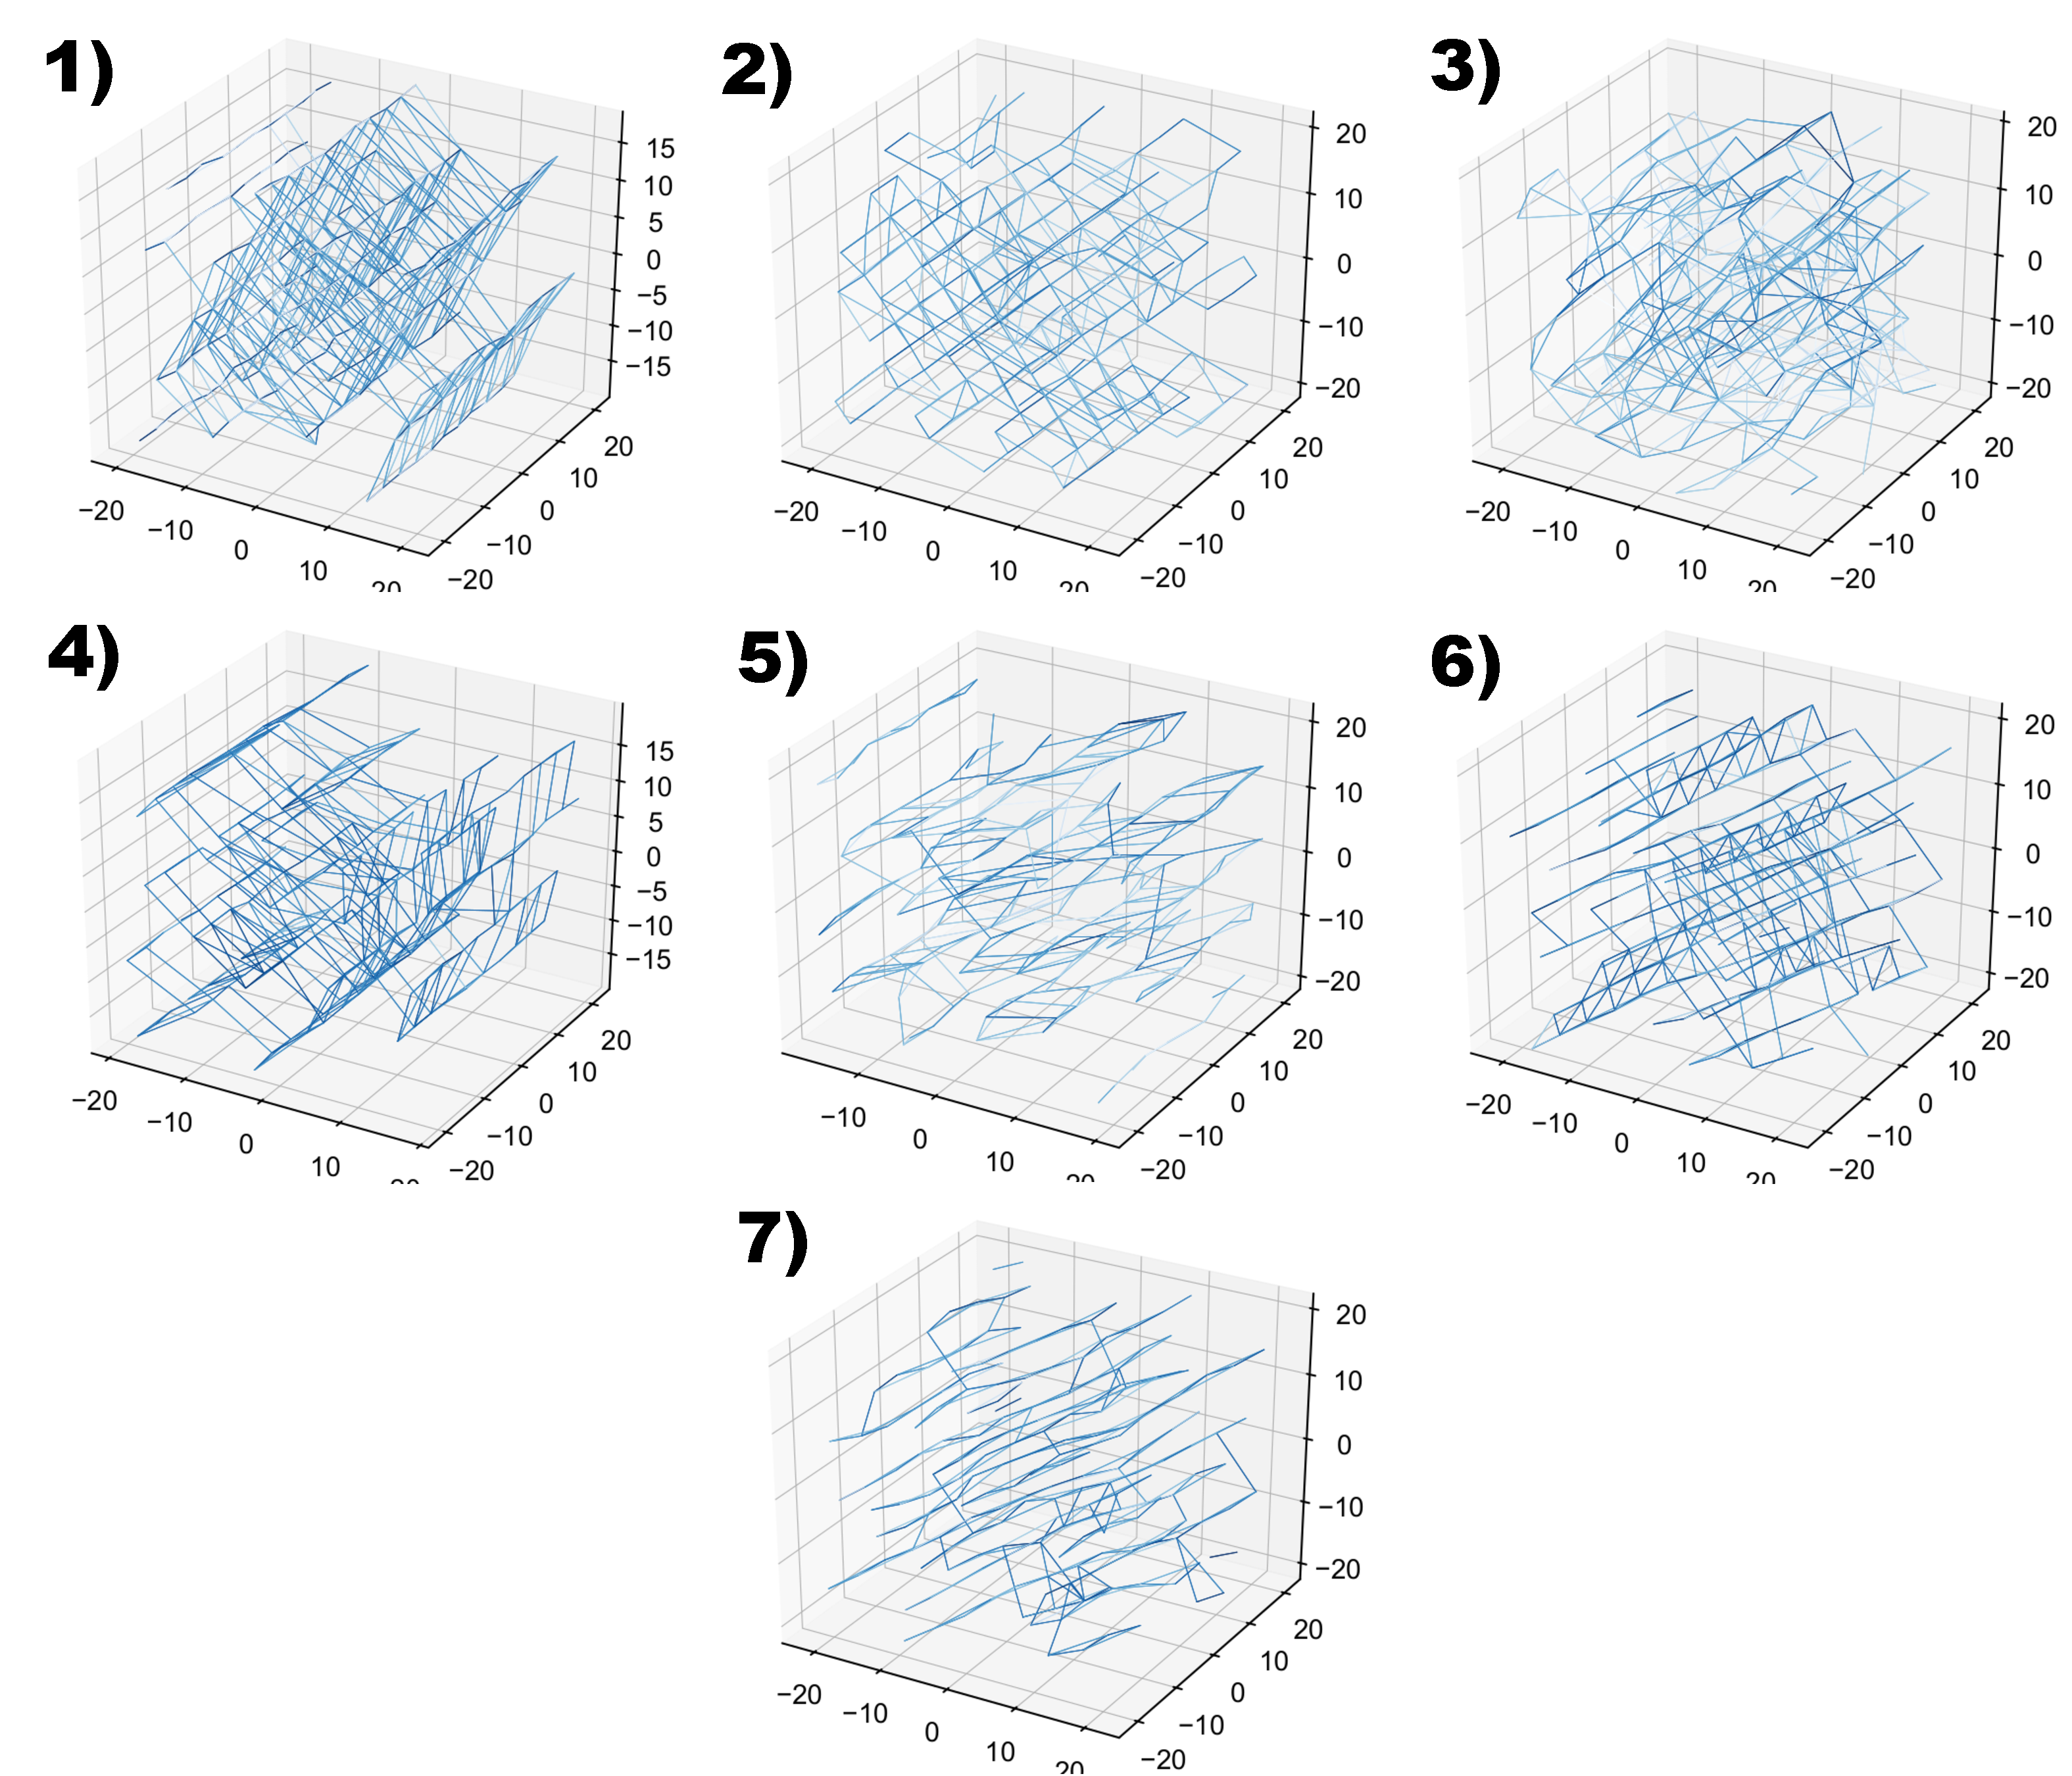
\includegraphics[width=\textwidth]{Figures/3dHole.pdf}
    \caption{The 3D heatmap of charge transport routes within the morphologies \textbf{1} - \textbf{7}.
    Dark routes describe commonly accessed hops between pairs of chromophores, whereas pale routes are less widely used in the KMC simulations.
    Each node therefore represents the location of a single chromophore.
The intensity value for the route is currently taken to be \texttt{I $=$ np.log10(freq) $/$ np.log10(max\_freq)}.}
	\label{fig:3dNetwork}
\end{figure}

\clearpage

\subsection{MSDs}

\begin{figure}[h!]\centering
	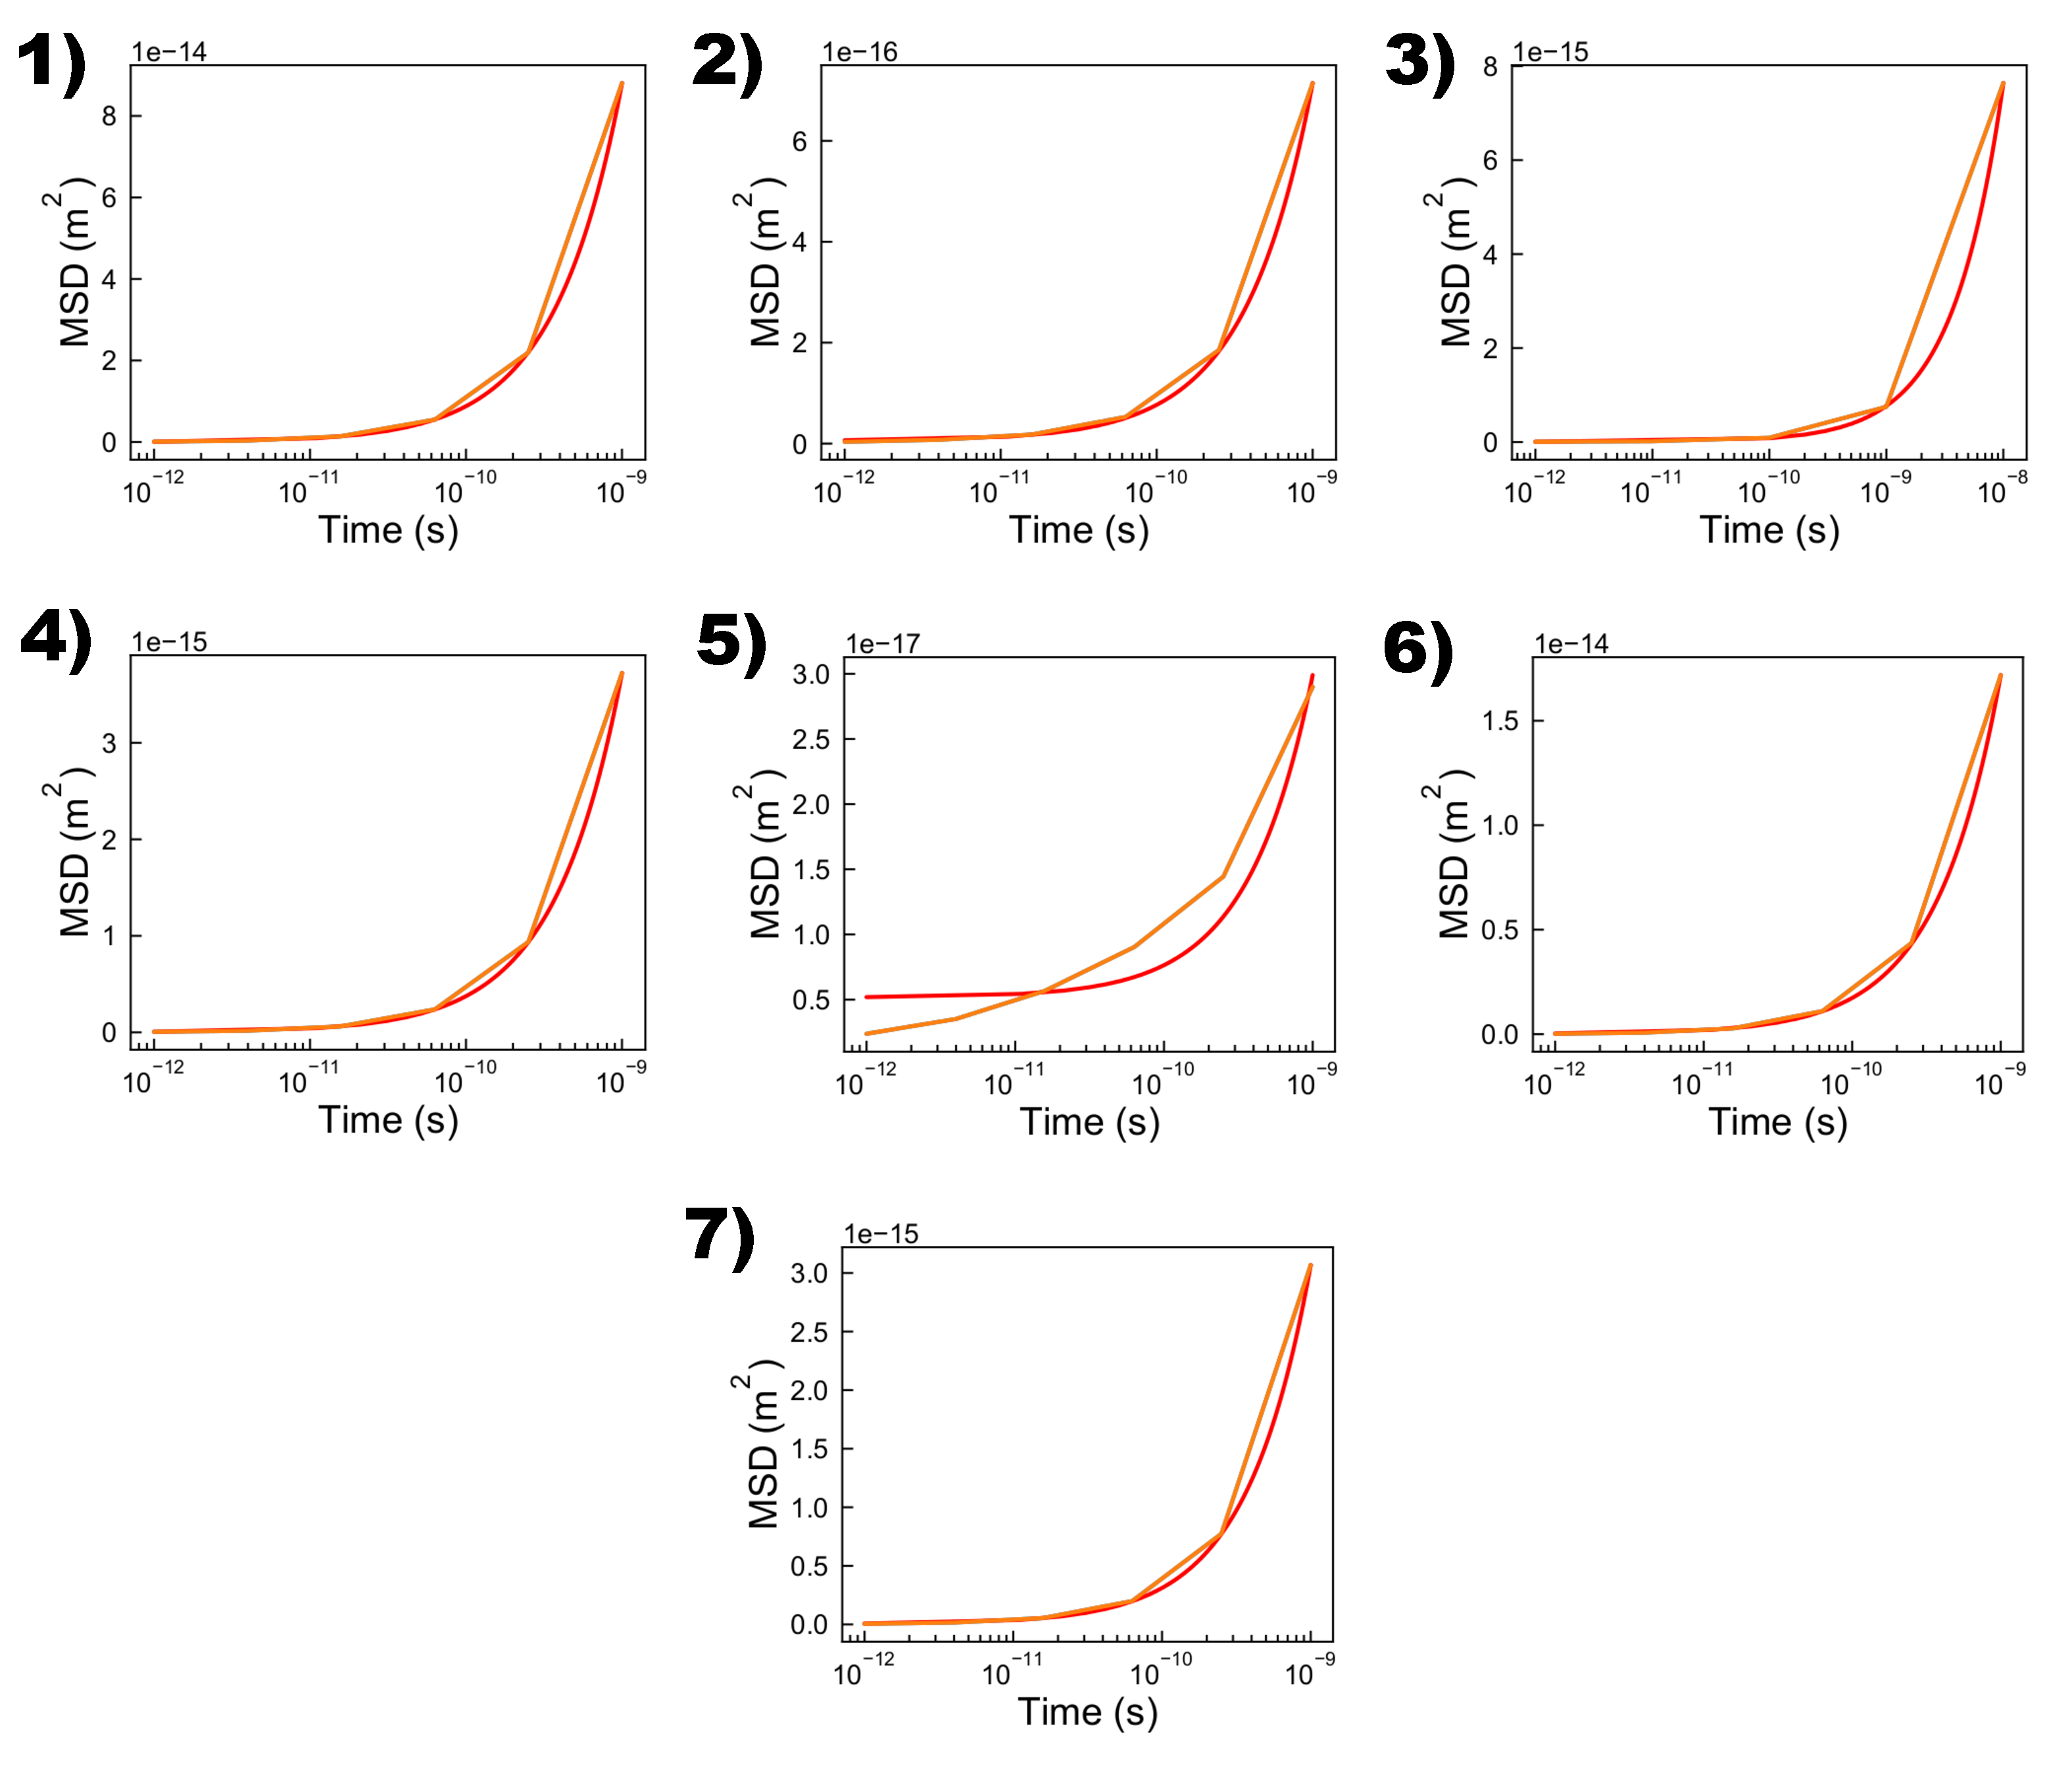
\includegraphics[width=\textwidth]{Figures/SemiLogMSDHole.pdf}
    \caption{The semi-log-x mean squared displacement curves of the carriers within the morphologies \textbf{1} - \textbf{7}.}
	\label{fig:MSD}
\end{figure}

\begin{itemize}
    \item{These are among the best fits we've ever had with MorphCT.}
    \item{The `odd one out' here is \textbf{5}, which exhibits slight saturation leading to a poorer fit.}
    \item{Fitting parameters have r values of > 99.999\%, except for \textbf{5} which has r = 97.29\%}
\end{itemize}

\clearpage

\subsection{Hopping Rate Distributions}

\begin{figure}[h!]\centering
	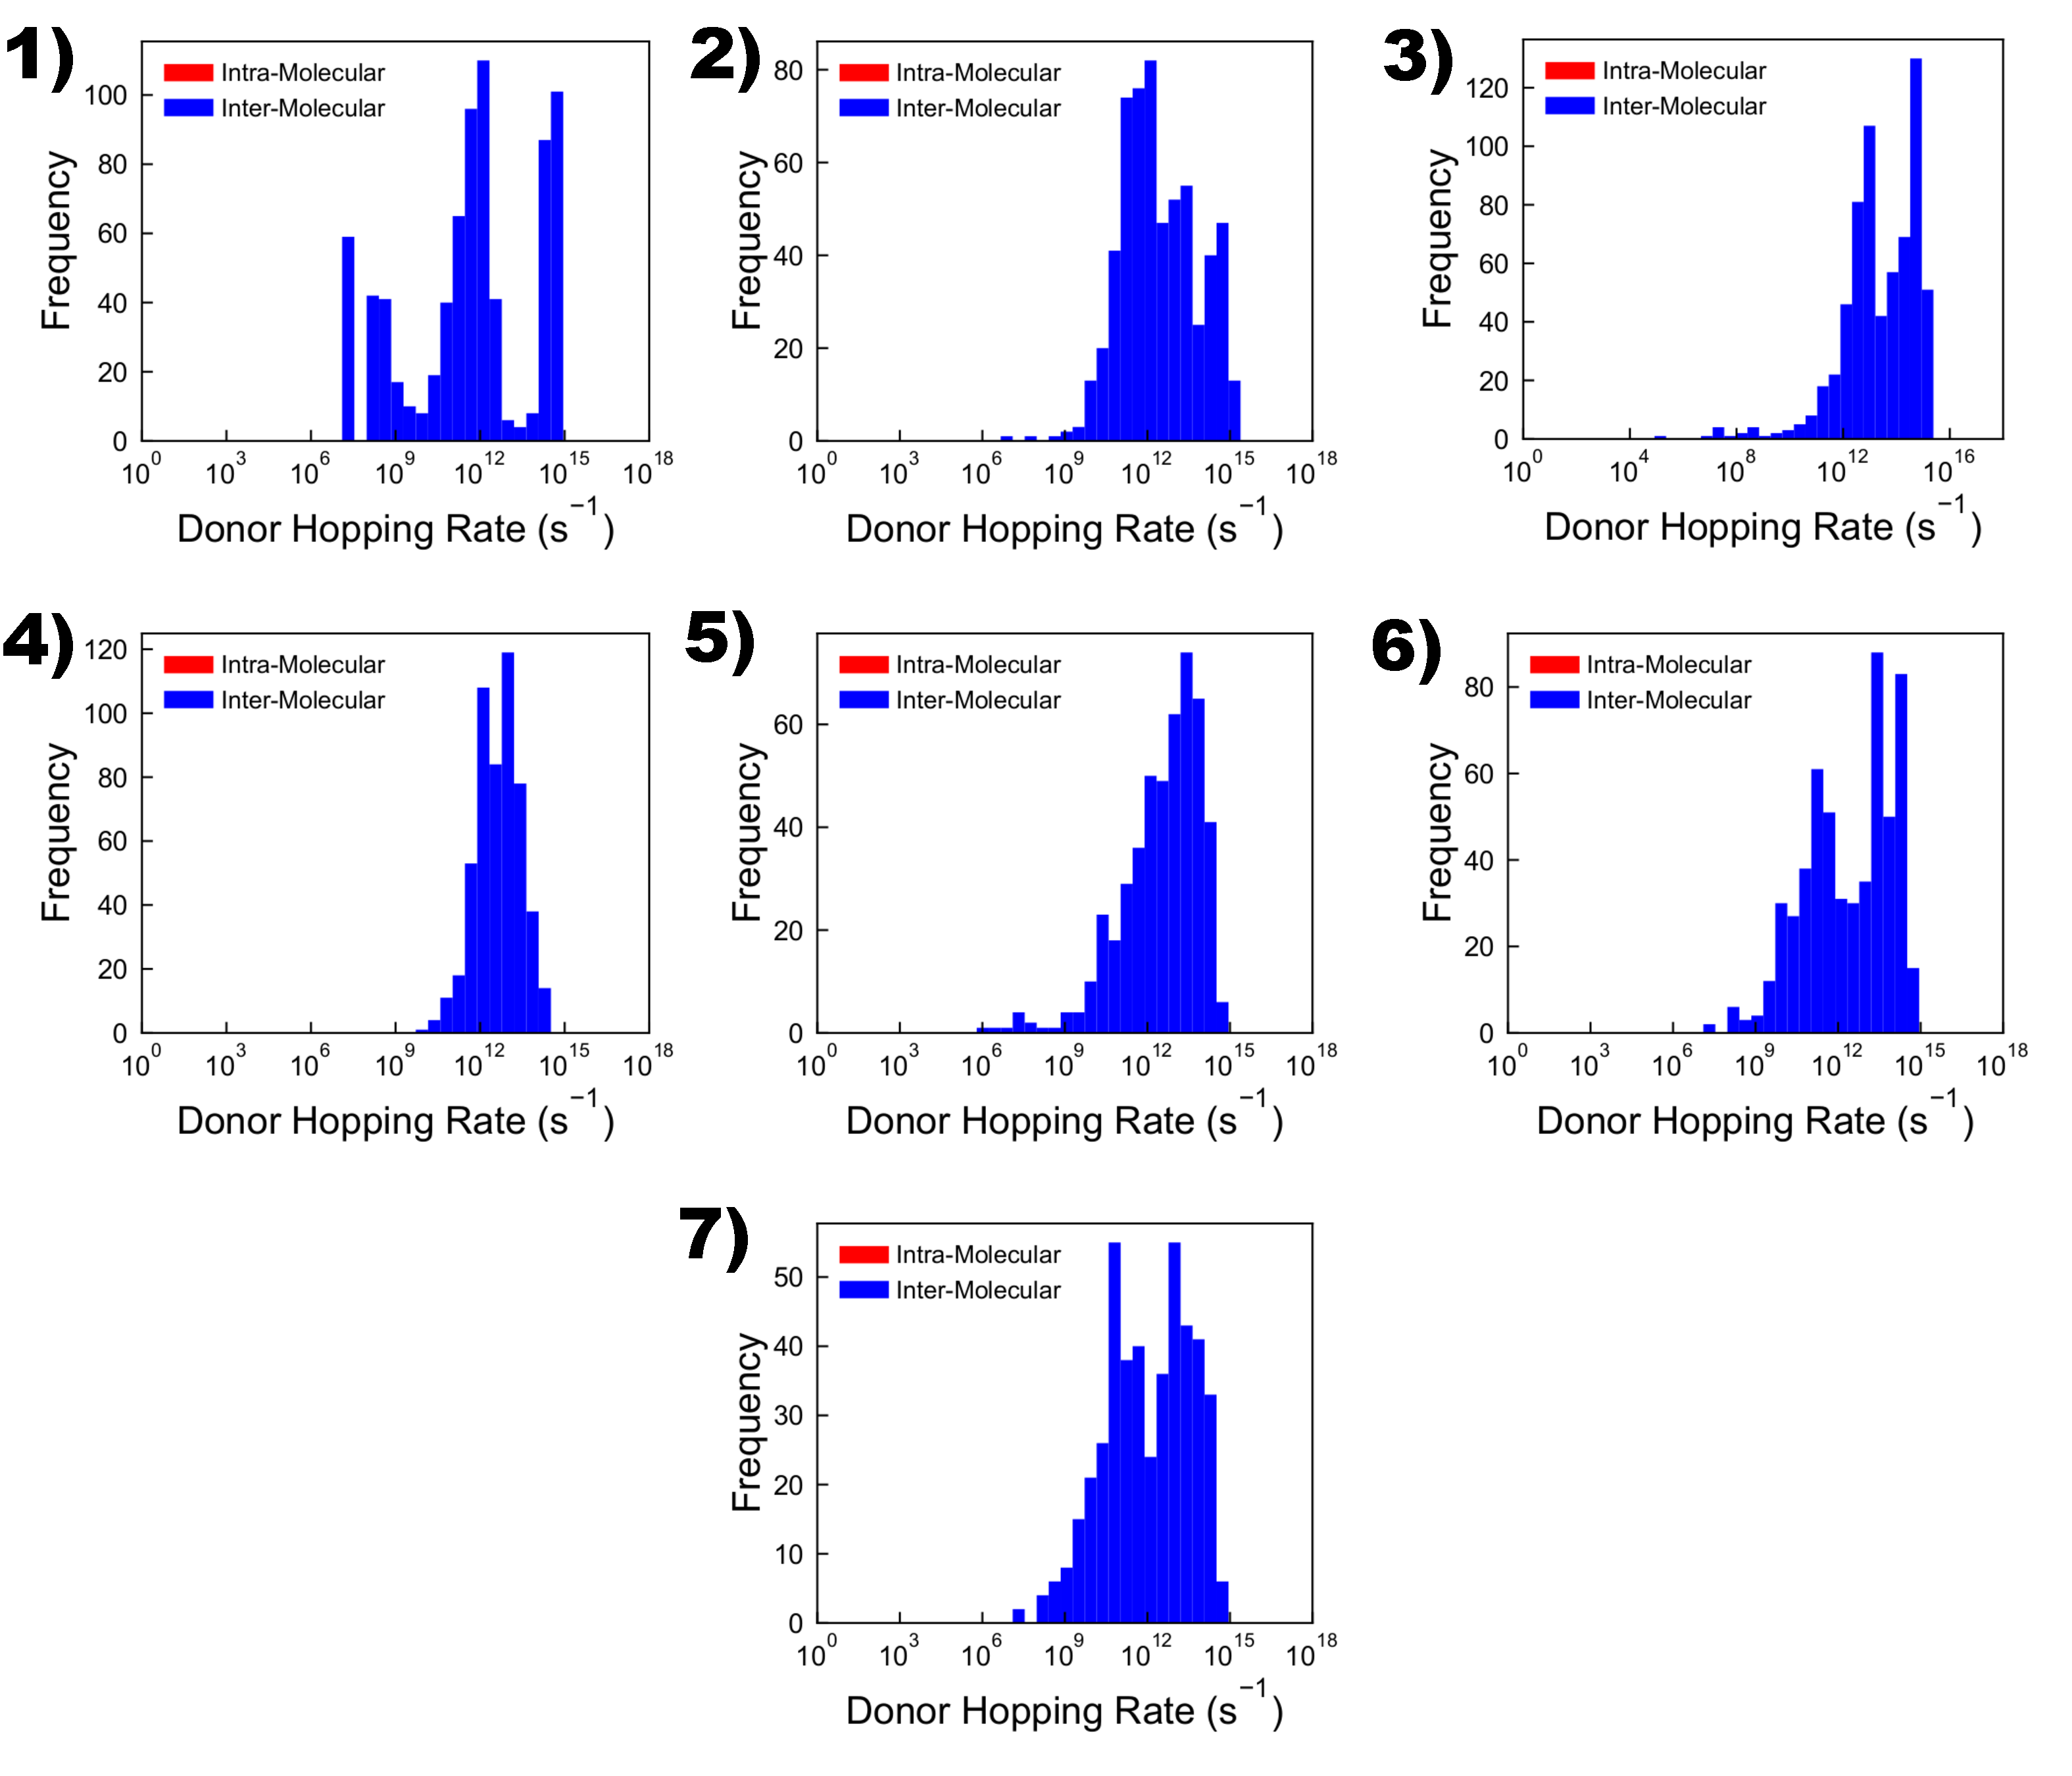
\includegraphics[width=\textwidth]{Figures/DonorHoppingRateMixed.pdf}
    \caption{The hopping-rate distributions for hops executed by carriers within the morphologies \textbf{1} - \textbf{7}.
    \textcolor{red}{It would require some pretty clever ad-hoc code, but it would be really nice to split this into intra- and inter-stack hops!}}
	\label{fig:HoppingRateMixed}
\end{figure}

\begin{itemize}
    \item{The hopping rate distributions vary quite a lot! Some are single-mode, others bimodal, and one is tri-modal.}
    \item{I will make more comments here after I've made the code mentioned above where we compare intra- to inter-stack hops}
\end{itemize}


\clearpage


\section{Outstanding Questions}


\begin{itemize}
    \item{TBA}
\end{itemize}


\bibliography{refs}
\bibliographystyle{unsrt}


\end{document}
